\startchapter{The Quark Framework}
\label{chapter:quark}

The Quark framework, also known as Open Quark, is a framework developed originally in the late 1990's at Business Objects.
It embodies a non-strict (lazy), strongly-typed functional language and runtime for the Java platform.  The main motivation behind the design of Quark was to create a system which allowed dual language development in which a functional language could be used to define declarative business models and these models could then be assembled by Java client programs responsible for user interfaces, communications protocols, interfacing to databases, security, legacy applications, and other applications for which Java proper was well-suited.  Thus it would allow a sort of ``meta-programming'', in a sense combining the best of both worlds (functional and object orientated) \cite{evans07}.  Quark itself consists of two main components:

\begin{itemize}
	\item CAL - a text-based functional language very much like Haskell
	\item The Gem Cutter - a visual programming environment based upon the CAL language
\end{itemize}

This thesis focuses on the latter of those two, the visual programming environment known as the Gem Cutter, however a cursory understanding of CAL will be helpful in understanding how the Gem Cutter works.  A brief overview of both follows, readers more interested in the details of Quark, CAL, and the Gem Cutter are referred to \cite{evans06, evans07}.

\section{CAL}

CAL is a non-strict (lazy), strongly-typed functional language, which targets the Java runtime.  That is, CAL source is compiled down to Java bytecode, and is it is thus possible to intermix components developed in CAL with components developed in Java proper.  In this sense it is very similar to the Scala programming language \cite{scala}.  It is even possible to call Java methods directly within CAL \cite{javaMeetsQuark}, however, obviously if one imports a functionally impure (ie - not referentially transparent) Java method, this compromises the purity of CAL as a whole (though in a very controlled way).  

Syntactically, CAL is very similar (and heavily inspired by) the Haskell programming language.  Like Haskell it makes full use of a Hindley-Milner type inference scheme, and implements essentially all the non-syntactic sugar features of Haskell 98. \cite{evans07, Ilic07}.  An example of some CAL source can be seen in \pref{prog:calmap} which shows the implementation of the functional programming staple function commonly called \code{map()} which given a function and a list of items, applies that function to each item in the list, returning the transformed list as a result.  

%That is, given a function \code{f()}, and a list L with items numbered from 0 through n, \code{map()} returns \code{f(L_0), f(L_1), ..., f(L_n)}.

\begin{program}
\begin{verbatim}
map :: (a -> b) -> [a] -> [b]; 
public map mapFunction !list = 
    case list of 
    []     -> []; 
    listHead : listTail ->  
        mapFunction listHead : map mapFunction listTail; 
    ; 
\end{verbatim}
\caption{The CAL Source Version of the map Gem}
\label{prog:calmap}
\end{program}

\section{The Gem Cutter}

\begin{flushright}
\textit{Full many a gem of purest ray serene\\
The dark unfathom'd caves of ocean bear:\\
Full many a flower is born to blush unseen,\\
And waste its sweetness on the desert air.}
\\
Thomas Gray \cite{Gray51} \\
\end{flushright}

In this section we shall introduce the Gem Cutter, and its interface, focusing on concepts that are directly related to exploring the environment from a pedagogical standpoint.  A full detailed technical description of the Gem Cutter can be found in \cite{evans07}, the ``official'' manual for the environment can be found at \cite{evans06}, and a simple tutorial on using the Gem Cutter designed for students in a third year software engineering course at the University of Victoria can be found at \cite{parkin08}.

The Gem Cutter is a visual interface to CAL code.  The interface allows one to create CAL functions called ``Gems'', which are directly translated into CAL source code, which is then in turn compiled and executed.  Thus, the Gem Cutter provides an environment in which one can explore the capabilities of CAL \emph{without writing a single textual line of code}.  This direct relationship between the visual reprsentation in Gem Cutter and the textual in CAL, and the teaching benefits that arise from this is one of the primary motivations behind this thesis.

The Gem Cutter starts up in a particular CAL workspace, where a workspace is a collection of CAL modules which form the initial environment for the Gem Cutter.  This start up window can be found in fixme reference.  The main interface of the Gem Cutter is made up of three components: the Scope Window which provides a tree-like overview of the gem currently being constructed, the Gem Browser which provides a list of all imported CAL modules for the current workspace, and the tabletop which is the area one composes (or ``cuts'') a new gem.

Interaction with the environment takes place by dragging and dropping various gems onto the tabletop, and connecting them together.  Each gem has a single output (on the right side of it), and an arbitrary number of inputs (depending on the gem in question) located on the left side.  Once a new gem has been constructed it can be saved, and then reused in new gem designs like any other predefined gem\footnote{Saved gems are by default stored in the GemCutterSaveModule module}.

We can also re-open a previously designed gem by right-clicking on the gem in the Gem Browser, and selecting ``Open Gem Design''.  Related to this feature, and an interesting consequence of the fact that Gems are just visual representations of CAL code, is that one can from within Gem Cutter view the corresponding equivalent CAL source code.  To do this, one right-clicks on the gem in the Gem Browser and selects ``Search For Definition'', upon which the interface will find the generated CAL source for the gem in question.  This is different from many other VPE's for which there is no direct equivalent textual form.  Note however, that while one can view the CAL source for any gem, the converse is not necessarily true.  Since many of the gems that are imported were written in CAL and not Gem Cutter, not all gems that are available in Gem Cutter have a gem design.

Like the VFPE described in \sref{sec:vpes}, the Gem Cutter essentially is a visual representation of the syntax tree of the program under construction.  Unlike the VFPE however, it uses a left to right rather than top-down orientation.  As well, the Gem Cutter allows one complete control over how gems are laid out on the tabletop.  This differs from the VFPE in which layout of components was done automatically by the environment.

\subsection{Useful Applications of the Gem Cutter}
\label{sec:gemCutterUsefulApps}

As a state-of-the-art visual programming environment based upon the functional paradigm, the Gem Cutter has a great deal to offer as a pedagogical tool in classroom environments.  In this section we outline some of the useful aspects of the environment.

\paragraph{Type Inference Permeates The Interface} 

Type inference can be confusing to new and old programmers alike.  It is difficult for new programmers because it is such an abstract concept.  It is difficult for older programmers well-versed in traditional statically-typed languages (like C++ or Java) to ``let go'' of the tendency to want to explicitly state a particular data type for an identifier\footnote{This is not without good reason, oftentimes programmers well versed in statically typed languages will think that a lack of programmer specified typing is equivalent to dynamic typing, and thus there is the fear of having type errors creep into their programs}.  The visual programming environment offered by Gem Cutter addresses both of these concerns: it allows for new programmers to interact with gems and see how the types of identifiers are inferred.  Furthermore, because type checking is enforced whenever connections between gems are made, it ``feels'' as though one is specifying types by making connections between gems, thereby alleviating concerns about the use of type inference.

\paragraph{Constrained Environment}

As with most visual programming environments, the Gem Cutter represents a relatively constrained environment compared to more traditional text-based programming environments.  Syntax errors are extremely difficult to produce\footnote{Unless one starts making use of code gems as then one is once again working in the textual domain}, as the structure of code is inherent and implied by the construction of gem graphs.  There is no need for statement terminators, there is never any ambiguity from dangling else/if-else clauses, nor is there every any confusion about which operation has greater precedence than another.  Furthermore, strict type-checking is enforced upon every connection, thus type errors are essentially removed.  As a result, students can focus more on problem solving and structuring solutions rather than fighting with minor syntactic issues.

\paragraph{Promotes Key Ideas In Programming}

Oftentimes instructors in first year programming classes have difficulty conveying some key concepts such as composition, encapsulation, and modular thinking to students.  Typically programming exercises in early programming classes tend to be small enough that the merits of modularity are not apparent, but rather seem like an artificial burden.  In Gem Cutter, each gem is categorized into different modules, making the problem of finding a particular gem far easier than would be the case if there was just a ``flat list'' of gems.  Thus the merits of modularity seem immediately apparent to students.  As well, in creating gems one often needs to \emph{compose} predefined existing gems together, and think of them in terms of opaque, ``black-box'' computational units (enforcing the idea of encapsulation).

\paragraph{Easy to Find Functions With Particular Type Signatures}

It is not uncommon for someone designing a learning exercise in the functional paradigm to reach a point where they require a function that has a particular type signature.  The Gem Cutter provides two main mechanisms for finding functions of a particular type: \emph{Intellicut} and \emph{The Gem Browser}.  

With Intellicut (seen in \fref{fig:intellicut}), when one hovers the mouse over a particular connection on a gem a small popup window will appear listing possible type-safe gems which can be linked to this connector.  Furthermore, there are three views in this popup, as one can select to see all valid gems, only the ``best'' gems, or a ``likely'' subset of gems.  This feature can oftentimes allow one to ``accidentally'' discover that perfect function to be used with many higher order functions such as \code{map()}.  From a learner's perspective, Intellicut provides a support mechanism which can help ``guide'' students to correct solutions without sacrificing learning objectives.  Intellicut is in many ways similar to syntax-directed editing, or code completion, where the goal is to simplify the development process by alleviating some of the cognitive load that programming entails.

%\insertFigureLoc{p}{6}{intellicut}{Intellicut showing the best 204 gems (left) and all 1,113 gems (right) for Map.find}

\begin{figure}[htp]
  \begin{center}
    \subfloat[Best 204 Gems for Map.find]{\label{fig:intel-a}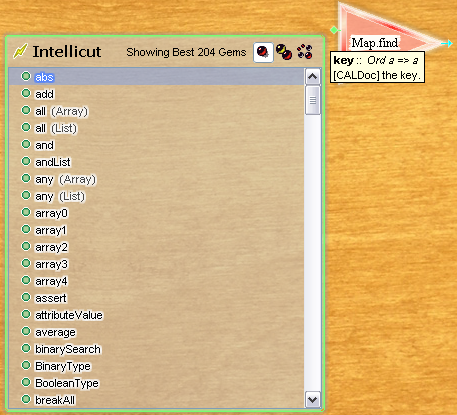
\includegraphics[scale=0.4]{Figures/intellicutBest}} \quad
    \subfloat[All 1,113 Gems for Map.find]{\label{fig:intel-b}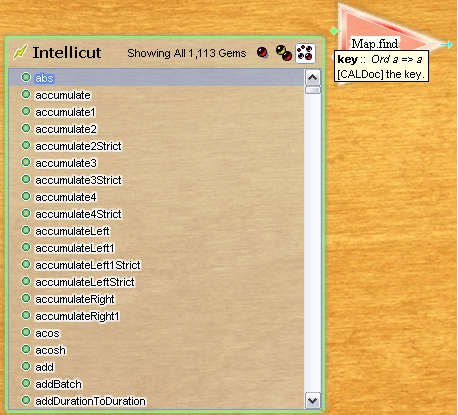
\includegraphics[scale=0.4]{Figures/intellicutAll}}
  \end{center}
  \caption{Using Intellicut to find gems}
  \label{fig:intellicut}
\end{figure}

With the Gem Browser, one can choose a variety of different groupings of gems.  The default is to group gems by Module, which is oftentimes the best, but it also allows one to group gems by type signature.  Both of these are seen in \fref{gemBrowserGroupings}, where on the left the default ``by module'' grouping is shown, and on the right the ``by gem type'' arrangement is shown.  There are additional browsing arrangements in addition to ``by module'' and ``by type'' including: by arity (number of arguments), by input type (essentially the same as ``by type'' but with return types removed), or by output type (essentially the same as ``by type'' but with input types removed).  Furthermore, for each arrangement, one can do a context-sensitive search to find exactly what one is looking for.  This can be seen in \fref{fig:gemBrowserGroup-b} where the results of a search for all gems which are of type \code{Num a => a -> a -> a} or ``all gems which take two numeric types and return a numeric type'' can be seen.

\begin{figure}[htp]
  \begin{center}
    \subfloat[Grouping by Module]{\label{fig:gemBrowserGroup-a}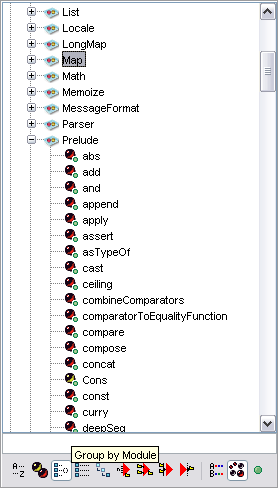
\includegraphics[scale=0.5]{Figures/gemBrowserGroupByModule}}\quad
    \subfloat[Grouping by Gem Type]{\label{fig:gemBrowserGroup-b}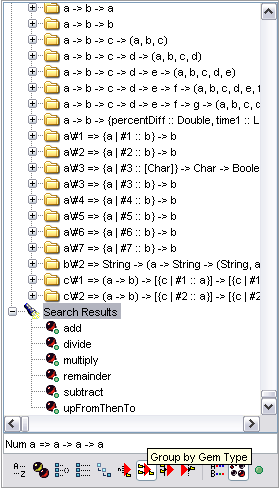
\includegraphics[scale=0.5]{Figures/gemBrowserGroupByType}}
  \end{center}
  \caption{Various gem groupings in the Gem Browser}
  \label{gemBrowserGroupings}
\end{figure}

\paragraph{Supports and Encourages Incremental Development}

At any point while developing a gem, one can right-click on that gem and select ``Run Gem'' to test out the partially constructed gem.  This is ideal for students, as at any point while they are working on a solution to a problem they can periodically test out parts of their design as needed to ensure that their gems work as intended.  That is, one does not have to create the entire solution before one can test out sub-parts of the solution.  Put another way, it encourages new programmers to ``test out'' small subsections of code, thereby making debugging easier and less time-consuming.

\subsection{Shortcomings of The Gem Cutter as a Learning Tool}
\label{sec:gemCutterShortcomings}

As mentioned, the Gem Cutter is a sophisticated tool that can be effectively used in learning environments.  However, given that it was primarily designed as a tool for software developers it is not surprising that there are some aspects of the Gem Cutter which could be improved to make it more suitable for use in an educational learning environment.

\paragraph{Single-User View}

The Gem Cutter generally has a single-user view of the world, which makes it difficult to effectively deploy in multi-user environments.  For example, in a Unix/Linux environment one typically wants to install an application in one central location, and have user-specific data saved into a user's \filepath{/home/username/} directory.  However, the current design of the Gem Cutter does not allow for this, the location of all user-generated data is stored within Gem Cutter's \filepath{/bin/} directory, thus one has to install the entire Quark framework separately for each individual user.  Furthermore, this structure of how user data is stored makes it difficult to move Gem Designs from one machine to another essentially requiring users to make a copy of the GemCutterSaveModule.cal file within the \filepath{/bin/cal/debug/CAL/} directory, along with all files in the \filepath{/bin/cal/debug/designs/-Gem-Cutter-Save-Module/} directory.  This is problematic for students who would like to bring work created in school labs to their home machines and vice-versa.

\paragraph{Inability to Create New Data Types}

There is currently no facility within the Gem Cutter to create new basic data types.  For example, when using the Word Game Framework, one may want to create a \code{GameState} type which is made up of a series of primitive data types (much like a \code{struct} in C).  However, as it stands now, the only way to do this is to create the data and type constructors for the new type in a separate CAL module, and modify the configuration files of the Gem Cutter to make use of this new module.  This significantly impacts the ability of instructors to make use of Gem Cutter to illustrate key ideas in functional type theory\footnote{Such as type and data constructors, parameterized types, type class constraints, and lacks contraints} as if one restricts themselves to only using the Gem Cutter, they can only supply pre-defined data types for students, rather than have students construct their own.

\paragraph{Difficult to Specify Types}

The Gem Cutter (like CAL) makes use of a very sophisticated type inference algorithm to infer the types of identifiers as needed.  This is useful, as it provides an excellent forum for illustrating the very interesting and useful programming language concept of type inference.  However, as is the case with any system which makes use of a type inference algorithm, it can sometimes be desirable to manually specify a specific type for an identifier.  This is certainly possible with CAL, for example if we want to say that an identifier ``x'' is a 2-tuple consisting of an Int and a list of Strings we would write \code{x :: (Int, [String])}.  However, from within Gem Cutter it can be difficult to enforce a particular type on a particular identifier.  Currently the easiest way to do this is to use a code gem and write an expression like the previously mentioned ``x'' declaration.  However, it would be preferable (and more within the visual programming paradigm) to perhaps right-click on a gem's connection and use the value editor seen with value gems to construct an explicit type.  This would be preferred from a teaching perspective in that much of the point of using a visual programming environment is to remove the possibility of syntax errors, whereas code gems are essentially windows into the world of text-based code writing, and thus allow for the possibility of syntax errors once again.\footnote{This is mitigated in code gems in that the code in a code gem is compiled immediately as one writes it, so at least syntax errors will be discovered very early on}

\paragraph{Inability to Open Multiple Gem Designs}

Currently the Gem Cutter can only work with a single gem design at at time.  This is somewhat awkward, as oftentimes (just like in the text-based paradigm) one will be working on a gem, and then want to modify or examine the implementation of another gem.  However, to do this one has to save the first (incomplete) gem, open up the other gem, then re-open the original gem.  As well, there are times when a not-yet-complete gem cannot be saved, so this requires arbitrary changes to the gem at hand to be able to save it before opening another gem design.

\paragraph{Dependencies Between Gems}
\label{para:Gemdependencies}

A rather significant shortcoming of the Gem Cutter is in regards to type dependencies between gems.  For example, if we create a gem called \code{foo} with type signature \code{String -> Int}, we can then make use of \code{foo} within another gem called \code{bar}.  If we then change the type signature of \code{foo} (say for example we decide we need Double precision numbers as the return type) we will in turn break the design of \code{bar}.  The Gem Cutter will produce an error message similar to that seen in \fref{depBreakErrMsg}.  Furthermore, and more seriously, we will likely cause problems within the Gem Cutter environment as a whole in that afterwords the GemCutterSaveModule module (where users save their gems) will no longer be accessible until one manually edits the underlying generated CAL code in GemCutterSaveModule.cal to remove or repair the definition of \code{bar} to be compatible with the new type signature of \code{foo}.  This might be reasonable for more ``seasoned'' computer science students, but it is probable that first year students will feel as though they damaged the environment and will in the future be more timid in attempting gem construction for fear of making the same (seemingly serious) mistake.

\insertFigure{4}{depBreakErrMsg}{The error message displayed by Gem Cutter when a type dependency is broken}

Furthermore, it is not only return types that cause this ``breakage'' to occur.  For example, if we have the same \code{foo()} gem as before, and we decide we need a second argument to \code{foo()}, we cannot simply add a second argument as if we do then the type of \code{bar()} will change as well.

To give an idea of how serious this problem is, note that the type dependency relationship between gems is transitive.  That is, if \code{a()} calls \code{b()} which calls \code{c()} which calls \code{d()}, then a change to \code{d()}'s type signature will break gems \code{a()}, \code{b()}, and \code{c()}.  This means that refactoring existing gems is extremely difficult as it means you have to first modify each gem to remove any dependencies between them, and then recreate the dependencies afterwords.  From an educational standpoint this is nearly a show-stopper, as students need to have the freedom to make design mistakes, and then go back and correct their mistakes, which is something the Gem Cutter currently does not easily allow, instead essentially requiring one to restart from scratch when a design mistake is found.


\paragraph{Difficult to Create New Modules}

The Gem Cutter makes use of a special module called \code{GemCutterSaveModule} and by default places all user-created gems into that module.  One can change this, and use a different \emph{already existing} module to save gems into, but there is no facility within Gem Cutter for creating a new module from scratch.  This would be desirable from a pedagogical perspective as it would allow one to better teach the concept of modularity in software design.  One can, however, create new modules by creating new CAL code modules in a text editor, and then add them to the current workspace.

\paragraph{Inability to Easily Remove Saved Gems}

Oftentimes when approaching a task for a first time a learner will make mistakes and want to start over from scratch.  In textual programming environments, this is easy -- just start with a new blank text file.  However, there is no mechanism within Gem Cutter for removing previously saved gems.  As it stands, the only way to remove saved gems is to manually edit the GemCutterSaveModule.cal file, removing the definition of the gem from that file, and then restarting the Gem Cutter.  For seasoned computer scientists this is relatively trivial (once you know where to look), but for new students of the discipline who are not yet conditioned or experienced with editing configuration files by hand, this can be a daunting task.  In either case it can be error prone, as if a removed gem is used in another gem's design, one can ``corrupt'' the workspace environment as seen in the ``Dependencies Between Gems'' section.  It would be preferred to have a more interactive mechanism, where one could right-click on a gem, pick ``Remove Gem'', and then the Gem Cutter could search all gem definitions to see if removing the gem should be permitted (\ie whether or not the gem to remove is used elsewhere).  Given that facilities for determining if gems are referenced inside other gems already exist within the Gem Cutter, it would appear that this should be a relatively small task to implement this additional functionality.

\paragraph{Using Non-Standard Modules}

A default, ``vanilla'' installation of the Quark framework will provide a Gem Cutter environment with most of the standard CAL modules available for use.  However, many of the modules which are available as part of the CAL language are not imported into the default Gem Cutter environment, instead appearing as ``greyed-out'' listings in the Gem Browser.  If one wants to use these modules within Gem Cutter they to either \begin{inparaenum}[\itshape a\upshape)]\item create a new workspace and select all the modules they want within that workspace\footnote{This can be done via the ``Workspace'' menu within Gem Cutter} or \item edit the GemCutterSaveModule.cal file by hand to import the module.\end{inparaenum}

\paragraph{Unfriendly Error Messages}

Particularly in regards to error messages, the Gem Cutter can produce alert windows that are not particularly friendly to users.  As an example, the author of this document once tried to modify the implementation of a previously created gem.  The original gem had the CAL source seen in \pref{prog:handleGuessedAlready}, and the gem layout seen in \fref{fig:handleGuess-a}:

\begin{program}
\begin{verbatim}
public handleGuessedAlready state =
    Cal.Core.Prelude.tuple2
        (
            (\s -> "\n\n ** You guessed this already! **\n\n" ++ s)
                (GemCutterSaveModule.displaySt state)
        )
        state
    ;
\end{verbatim}
\caption{The CAL Source Version of the handleGuessedAlready Gem}
\label{prog:handleGuessedAlready}
\end{program}


\begin{figure}[htp]
  \begin{center}
    \subfloat[The Initial Implementation of the handleGuessedAlready Gem]
    	{\label{fig:handleGuess-a}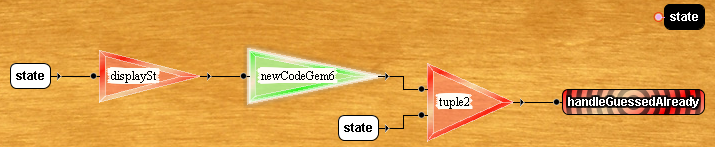
\includegraphics[width=4in]{Figures/handleGuessedAlreadyImpl}}\\
    \subfloat[The Second Implementation of the handleGuessedAlready Gem]
    	{\label{fig:handleGuess-b}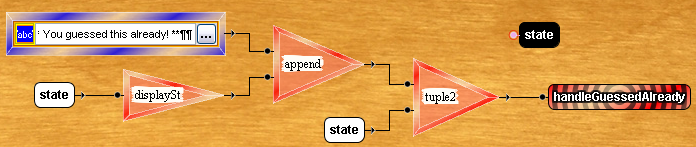
\includegraphics[width=4in]{Figures/handleGuessedAlreadyImplNew}}
  \end{center}
  \caption{Two Versions of the handleGuessedAlready gem}
  \label{fig:handleGuessedAlready}
\end{figure}

\begin{figure}[htp]
  \begin{center}
\begin{verbatim}
An error condition was flagged whilst compiling the test.
The captured error text was:
Error: GemCutterSaveModule: The declared type of the function 
cdlInternal_runTarget is not compatible with its inferred type 
(a\#1, a\#2, a\#3) => {a | #1 :: Cal.Core.Prelude.String, #2 :: 
Cal.Core.Prelude.Int, #3 :: [Cal.Core.Prelude.Char])} -> 
(Cal.Core.Prelude.String, {a | #1 :: Cal.Core.Prelude.String, 
#2 :: Cal.Core.Prelude.Int, #3 :: [Cal.Core.Prelude.Char]}). 
Caused by: record type unification failed at field #2. Attempt 
to instantiate a record variable from the declared type.
\end{verbatim}
\end{center}
  \caption{A Lengthy Type Error Message Produced by the Gem Cutter}
  \label{fig:longErrMsg}
\end{figure}

It was modified to remove the code gem which appended two strings together to instead explicitly use the \code{append()} gem in the Prelude module.  The new layout can be seen in \fref{fig:handleGuess-b}.  However, after doing this and then running the new gem layout the Gem Cutter once produced the error message seen in \fref{fig:longErrMsg}.  This was problematic from the perspective of new programmers for a few reasons:

\begin{itemize}
	\item It uses technical and cryptic language (what is meant by ``instantiate a record variable from the declared type''?)
	\item The record type notation, along with the explicit type specifiers make it difficult to pull out key information
	\item There are ``magic'' names in the message (for example, cdlInternal\_runTarget is the name given to the compiled gem when one tries to run a partial gem layout)
	\item The entire error message appeared in a single line which meant that the dialog window that contained the error message was 2,419 pixels wide, which would not fit on even a very high resolution screen.
	\item Most importantly, there should not have been an error, as visually, one was simply connecting the output of two gems into the \code{tuple2()} gem, which should accept two items of \emph{any} type.  After placing a code gem which explicitly specified a type for the ``state'' parameter\footnote{It was a 3-tuple of type \code{(String, Int, [Char])}} the error message ceased to appear (even after the code gem was removed).
\end{itemize}

\paragraph{No Visual Facility for Lambda Expressions}

As it stands the only way to create an unnamed function or lambda expression is to use a code gem.\footnote{In fact, a code gem really is a lambda expression, as while they can be named the name is purely for documentation purposes}  While not a problem from a practical point of view, it is difficult to convey to learners the theoretical background of functional programming\footnote{The Lambda Calculus} without discussing lambda expressions.

\paragraph{Poor Documentation}

Being a relatively newly open-sourced project\footnote{The OpenQuark framework was released under a BSD-style license on January 25, 2007 \cite{bobjNews}}, there is not yet a great deal of user-friendly documentation available.  Currently the only real documentation on the Gem Cutter consists of \cite{evans07} and \cite{evans06}.  The former is a conference-style technical paper, and the latter is more of an overview of features with little detail on how to resolve problems within the environment.  There is however, a community dedicated to providing assistance via the CAL Language Discussion Google Group\footnote{Found at: \url{http://groups.google.com/group/cal_language}}.  This document is the first work we have found which addresses the Gem Cutter from an educational usage standpoint.

\paragraph{Confusion Between Records and Tuples}

In CAL, tuples are treated as records with the first field named \code{\#1}, the 2nd \code{\#2}, etc.  This seems natural, however, it can lead to some confusion in terms of type specifiers.  For example, a record consisting of an Int in field \code{\#1}, and a String in \code{\#2} would be of type:

\verb!(a\#1, a\#2) => {a |#1 :: Int, #2 :: String}!

However, this looks quite different than \code{(Int, String)}, even though the two types are equivalent.  This can be a source of confusion for students not well-versed in various compound type schemes.  An example of this is seen in \fref{tuplevsrecord} where we have a \code{tuple2()} gem and a \code{field1()} gem.  The output of \code{tuple2()} is completely type equivalent to the input of \code{field1()}, even thogh the type identifiers look quite different (particularly to the untrained eye).

\insertFigure{3}{tuplevsrecord}{The tuple2 and field1 gems}
